\chapter{Logical Operators}\label{CHAP_LogicalOperators}

\section{Difficulty: EASY}


\subsubsection*{Exercise 5.E01}
Complete the following so-called truth table.
\begin{figure}[H]
		\centering
		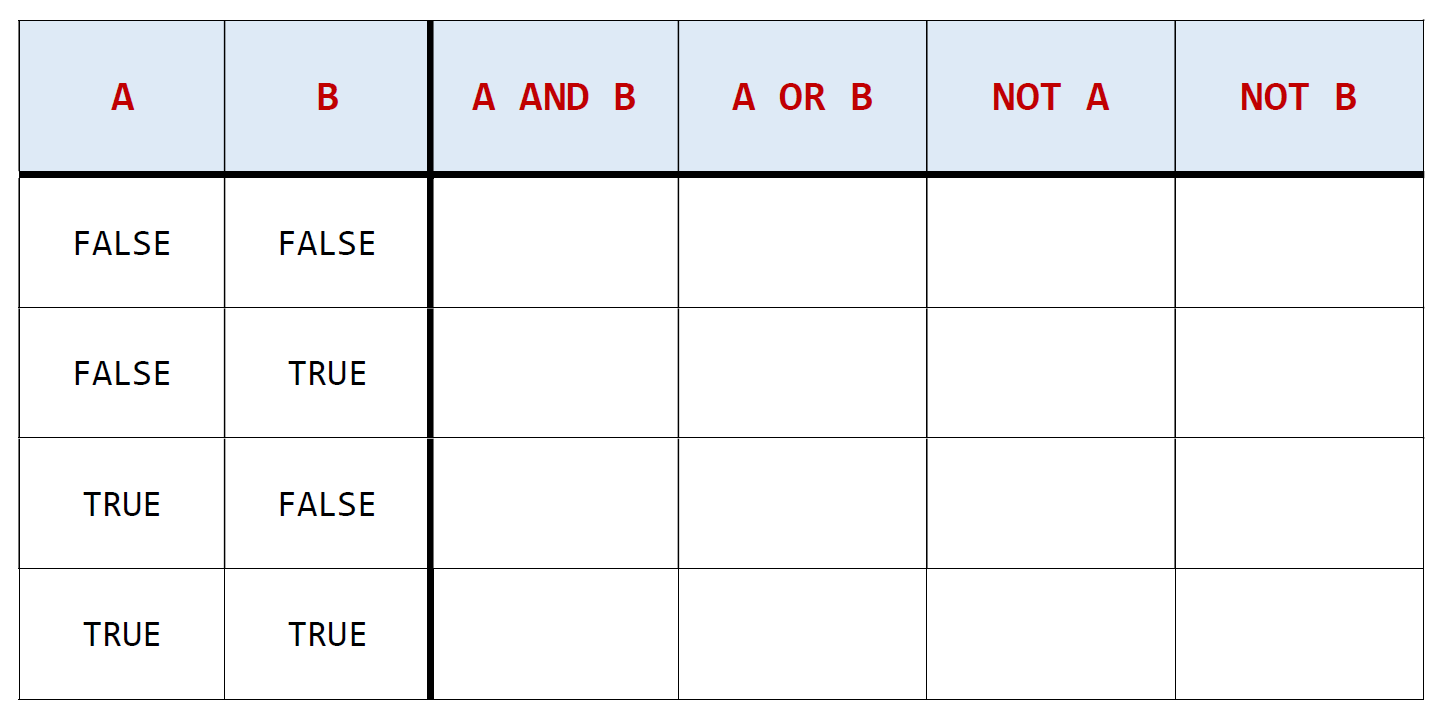
\includegraphics[width=\textwidth]{../IMG/5E01.png} 
\end{figure}


\textit{Hints:
You can use this table throughout the remainder of the course whenever you need to
generate conditional cases using logical operators!}\\[1cm]


% ------------------------------------------------------------------------------
\newpage
\subsubsection*{Exercise 5.E02}
Consider the variables:
\begin{figure}[H]
		\centering
		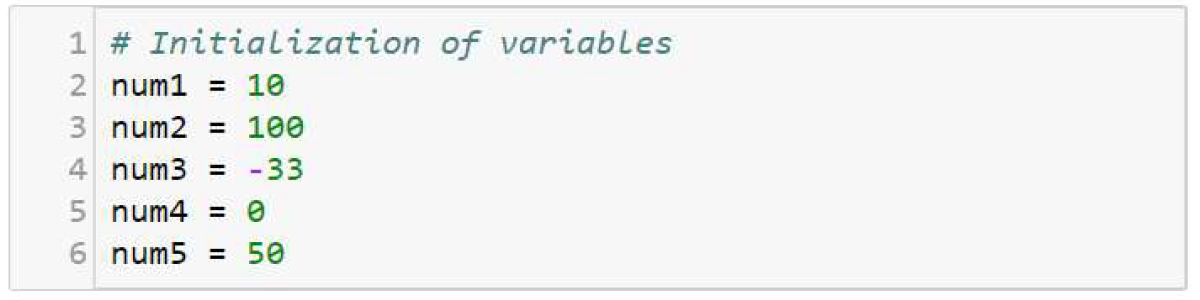
\includegraphics[width=\textwidth]{../IMG/5E02.png} 
\end{figure}
and evaluate the following expressions:
\begin{enumerate}[label=(\alph*)]
	\item {\code{(num1 > num2) or (num3 > num4)}}
	\item {\code{(num1 != num3) and (num4 < num5)}}
	\item {\code{((num4 + num5) > 0) or (num2 < num3)}}
	\item {\code{not (num2 == num4)}}
\end{enumerate}
	
\textit{Hints:
You can solve this exercise on the exercise sheet. If you’re struggling to get started, copy the command lines into a Jupyter Notebook and execute the code. You can also try copying the commands onto a piece of paper and colouring corresponding brackets in the same colour.}\\[1cm]


% ------------------------------------------------------------------------------

\subsubsection*{Exercise 5.E03}
Simplify the following logical expressions for an arbitrary Boolean bol:
\begin{enumerate}[label=(\alph*)]
	\item {\code{bol and False}}
	\item {\code{bol or False}}
	\item {\code{bol and True}}
	\item {\code{bol or True}}
	\item {\code{not (not bol)}}
\end{enumerate}

\textit{Hints:
You can solve this exercise on the exercise sheet. If you’re struggling to get started, copy the command lines into a Jupyter Notebook and execute the code for some examples of {\code{bol}}.}


% ------------------------------------------------------------------------------

\newpage
\section{Difficulty: MEDIUM}

\subsubsection*{Exercise 5.M01}
Consider the following piece of code:
\begin{figure}[H]
		\centering
		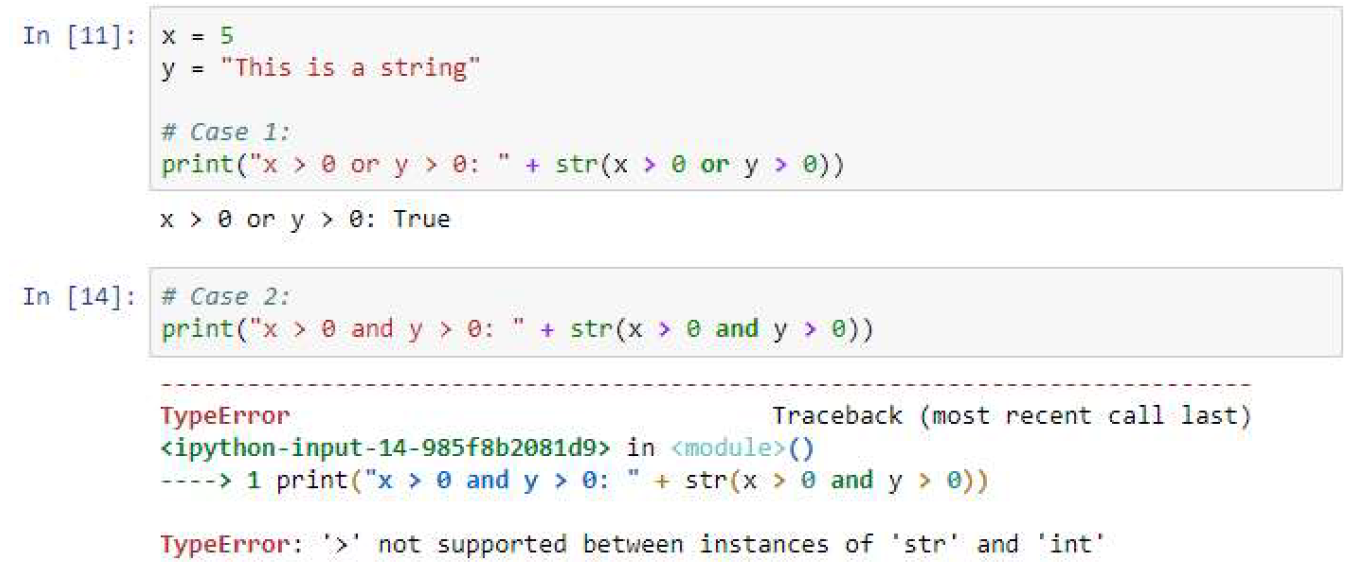
\includegraphics[width=\textwidth]{../IMG/5M01.png} 
\end{figure}
The operation {\code{y > 0}} is invalid because {\code{y}} is a string and {\code{> a}} mathematical operator.\\
Why is Case 1 executed without a problem while Case 2 results in an error message?\\

\textit{
Hints:
Consider the different behaviour of the {\code{AND}} and the {\code{OR}} operator when they encounter one {\code{TRUE}} statement.}\\[1cm]


% ------------------------------------------------------------------------------

\subsubsection*{Exercise 5.M02}
Starting with the following variable definitions:
\begin{figure}[H]
		\centering
		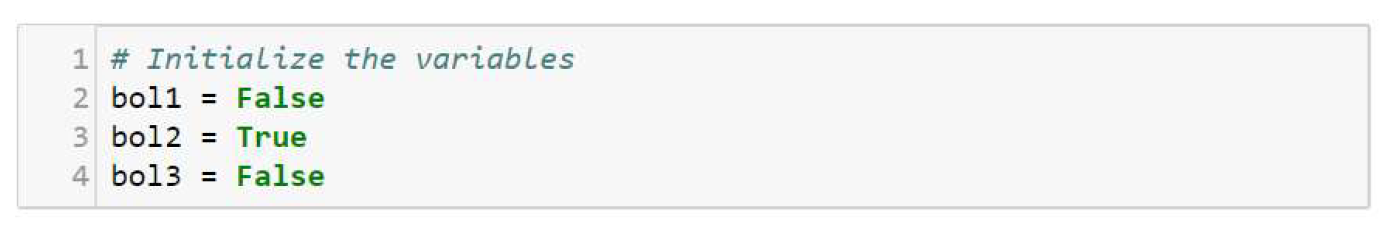
\includegraphics[width=\textwidth]{../IMG/5M02.png} 
\end{figure}
Determine the value of:
\begin{enumerate}[label=(\alph*)]
	\item {\code{bol4 = bol1 or bol2 and not bol3}}
	\item {\code{bol5 = not bol1 and bol3 or bol2}}
	\item {\code{bol6 = not(bol2 or bol3)}}
	\item {\code{bol7 = not(bol2 and not bol3)}}
	\item {\code{bol8 = not(bol1 or bol2) or (bol2 and bol3)}}
	\item {\code{bol9 = bol1 or (bol1 or (bol1 or bol2)) or bol3}}
	\item {\code{bol10 = bol9 and bol2 and not bol3}}
\end{enumerate}


\textit{Hints:
You can solve this exercise on the exercise sheet. If you’re struggling, try copying the relevant lines into Jupyter Notebook and execute them step by step.}\\[1cm]


% ------------------------------------------------------------------------------

\subsubsection*{Exercise 5.M03 \red{[M]}}
Starting with the following variable definitions:
\begin{figure}[H]
		\centering
		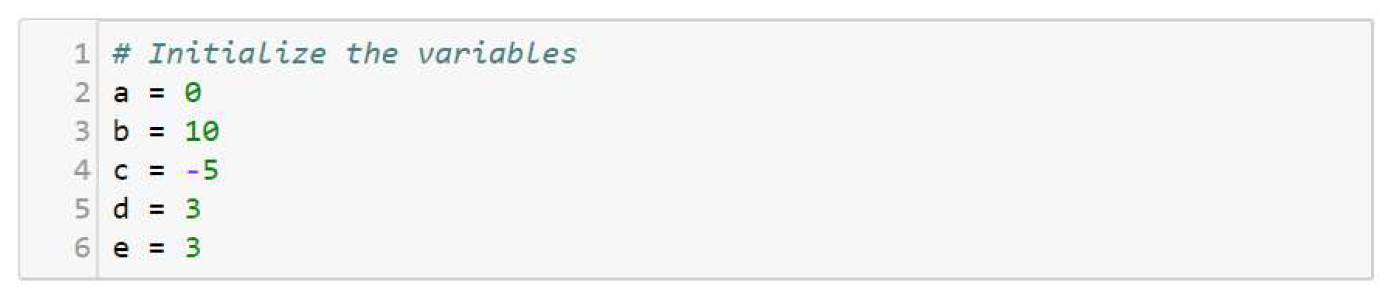
\includegraphics[width=\textwidth]{../IMG/5M03.png} 
\end{figure}
Determine the expressions::
\begin{enumerate}[label=(\alph*)]
	\item {\code{bol1 = a > b or a > c}}
	\item {\code{bol2 = a == 0.0 or d == 4.9}}
	\item {\code{bol3 = c < -6 or (d > 0 and e == d)}}
	\item {\code{bol4 = a + b <= 11 or d == 5}}
	\item {\code{bol5 = not (a > 30 or d < 0)}}
	\item {\code{bol6 = not (not (not (a + e > 2 or c + b > 0) or e – a > 2))}}
	\item {\code{bol7 = not (b\%2 == 0)}}
	\item {\code{bol8 = (c\%2 > 0 or e\%2 > 0 or b\%2 > 0) and a\%4 == 0}}
	\item {\code{bol9 = (b//2 > 0 and not(a//2 > 0)) or (not(b//2 > 9) and a//2 > 0)}}
	\item {\code{bol10 = not (bol3 and (a + b**2 > 50)) or d == e}}
\end{enumerate}

\textit{Hints:
You can solve this exercise on the exercise sheet. If you’re struggling, try copying the relevant lines into Jupyter Notebook and execute them step by step.}\\[1cm]


% ------------------------------------------------------------------------------

\subsubsection*{Exercise 5.S01}
For the initial values:
\begin{figure}[H]
		\centering
		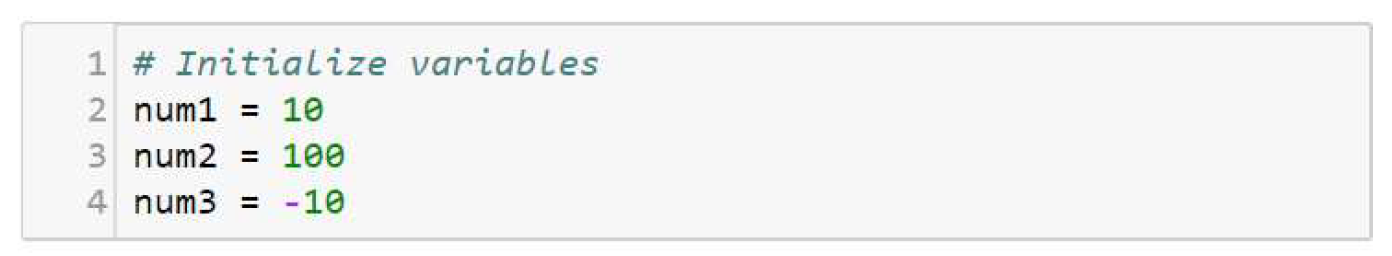
\includegraphics[width=\textwidth]{../IMG/5S01.png} 
\end{figure}
and without copying the commands into Jupyter Notebook, evaluate the following
expression:
\begin{center}
	{\code{bol = num1 > num2 and num2 > num3 or num3 > num1}}
\end{center}


\textit{Hints:
Logical operators are easier to determine with brackets. Insert brackets in above expression and then evaluate one expression at a time starting with the innermost bracket until the entire command line is reduced to a Boolean.}\\[1cm]


% ------------------------------------------------------------------------------

\subsubsection*{Exercise 5.S02}
For the initial values:
\begin{figure}[H]
		\centering
		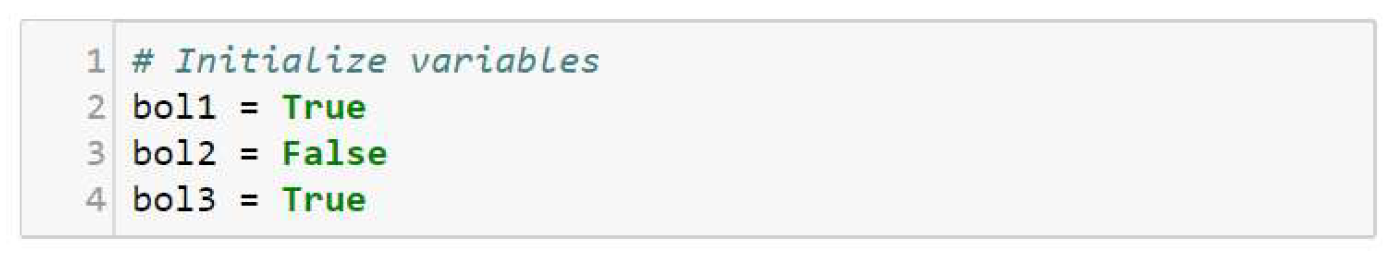
\includegraphics[width=\textwidth]{../IMG/5S02.png} 
\end{figure}
and without copying the commands into Jupyter Notebook, evaluate the following
expression:
\begin{center}
	{\code{bol = bol1 or bol2 or bol3 and not bol1}}
\end{center}


\textit{Hints:
Logical operators are easier to determine with brackets. Insert brackets in above expression and then evaluate one expression at a time starting with the innermost bracket until the entire command line is reduced to a Boolean.}


% ------------------------------------------------------------------------------

\newpage
\section{Difficulty: HARD}

\subsubsection*{Exercise 5.H01}
You can build all kinds of complex logical operators using combinations of {\code{AND}}, {\code{OR}} and {\code{NOT}}. In fact, you can even construct the {\code{AND}} operator using only {\code{OR}} and {\code{NOT}} and the {\code{OR}} operator using only {\code{NOT}} and {\code{AND}}.\\
In this exercise you won’t have to write any code. Instead try and find a way to
\begin{enumerate}[label=(\alph*)]
	\item Rewrite {\code{statement1 and statement2}} using only {\code{OR}} and {\code{NOT}}
	\item Rewrite {\code{statement1 or statement2}} using only {\code{NOT}} and {\code{AND}}
\end{enumerate}
	
\textit{Hints:
You will need several instances of the operators in each case. Try starting with a fixed set of statements and try adding operators to obtain the result you want.}
